\chapter{Tests}
\label{cha:test}

 In order to be able to tell specimen apart quickly, the following naming convention was followed.

\section{Naming Convention}

A specimen name is assembled as follows:


\centering
\textbf{date\_description\_thickness[mm]\_energy level [kJ](\_repetition number)}
\flushleft

\subsection*{Date}

The international standard date notation is used. Year-Month-Day.

\subsection*{Description}

\begin{table}
\centering
\begin{tabular}{lr}
\toprule
Description & Shorthand \\
\midrule
plain shotcrete & s\\
fibre reinforced shotcrete & frs \\
welded mesh reinforced shotcrete & mrs \\
chain-link mesh reinforced shotcrete & crs \\
textile mesh reinforced shotcrete & crs \\
\hline
welded mesh underneath & + w \\
chain-link underneath & + c \\
textile mesh & + t\\
fjällband underneath & + j\\
lacing underneath & + l\\
TSL underneath & + s\\
\bottomrule
\end{tabular}
\caption{Sample description}
\label{tab:samdes}
\end{table}
%As of yet only round frs samples have been tested. So this section of the name starts with R to mark round samples and continues with frs to denote the composition. All current samples therefore have the same notation: Rfrs.

The description of the specimen is slightly more complicated, it was developed to be able to be used in future tests as well and is over complete. The first part is the test method:

\begin{itemize}
    \item dynamic tests are not marked (standard)
    \item \textbf{Q} marks quasi-static tests
    \item \textbf{C} marks samples that were tested quasi static after a dynamic test (combination)
\end{itemize}

The next part is the sample shape.

\begin{itemize}
    \item square samples are not marked (standard)
    \item \textbf{W} marks square samples without adhesion to the concrete slab
    \item \textbf{R} marks round samples
\end{itemize}

Lastly the composition of the panel, as described in \autoref{tab:samdes}. Please note that the composition is named starting from top to bottom. 


\subsection*{Energy Level}

The energy levels are given in kJ and are rounded to one decimal place and calculated using \(E_{pot} = m * g *h \), with \(g =9,8~\frac{\text{m}}{\text{s}^2}\). %Of course some of this calculated energy is dissipated, for example through vibrations of the rig and bouncing of the impact weight. The exact amount of energy absorbed by the specimen is therefore unknown.

This naming scheme fails for test that have been subjected to multiple impacts. for the tests both the total energy input and the impact are required. This can be achieved by writing XmY, with X denoting the energy of the impact and Y the total energy input into the panel.

\subsection*{Number of Repetitions}

The number of repetition is only used for the second and following repetitions. Therefore the first sample of a given composition is not marked especially. This makes it easier to spot tests with several repetitions.

\subsection*{Examples}

\centering
\textbf{19-06-21\_Qs+m+j+j\_150\_0\_3}
\flushleft

Would be a quasi-static test run on 2019-06-21 on a square specimen, made of plain shotcrete that has external mesh and two layers of Fjällband and is plain shotcrete. The specimen has a thickness of 150 mm, as the test is quasi-static the energy level is zero, and it is the third test run in this setup on that day.

\medskip
\centering
\textbf{18-12-04\_Rfrs\_50\_0,3}
\flushleft

Would be a test run on 2018-12-04 on a round specimen made from fibre reinforced concrete with a thickness of 50 mm, an energy level of 0,3 kJ and it would be the first test in this setup.


The tests were spaced out over a long time span and the sensor array changed several times during testing. In \autoref{tab:con} an overview of the different testing conditions is given. 


\begin{table}
    \centering
\begin{tabular}{l l l l l l l}
\toprule
Name & Number & Energy level & Thickness & Drop weight & Drop height &  Age \\
                         &        &              &           &             &             &      \\
\midrule
2017-12-20\_Rfrs\_75\_1,8       &      1 &         1.76 &        75 &         200 &       899.3 &      \\
2017-12-20\_Rfrs\_75\_3,5       &      2 &         3.53 &        75 &         200 &      1799.1 &      \\
2018-02-14\_Rfrs\_75\_1,0       &      3 &         0.98 &        75 &         100 &         997 &   16 \\
2018-02-14\_Rfrs\_75\_0,5       &      4 &         0.49 &        75 &         100 &       496.7 &   16 \\
2018-11-09\_Rfrs\_75\_0,5       &      5 &         0.49 &        75 &         100 &       500.3 &  133 \\
2018-11-29\_Rfrs\_75\_1,0       &      6 &         0.98 &        75 &         100 &       998.8 &  137 \\
2018-12-04\_Rfrs\_50\_0,7       &      7 &         0.66 &        50 &         100 &       672.3 &  158 \\
2018-12-04\_Rfrs\_50\_0,3       &      8 &         0.29 &        50 &         100 &       299.3 &  158 \\
2018-12-04\_Rfrs\_50\_0,3\_2     &      9 &         0.29 &        50 &         100 &       299.3 &  158 \\
2018-12-10\_Rfrs\_100\_2,0      &     10 &         1.95 &       100 &         100 &      1990.4 &  164 \\
2018-12-10\_Rfrs\_100\_1,5      &     11 &         1.47 &       100 &         100 &      1501.5 &  164 \\
2018-12-10\_Rfrs\_100\_1,5\_2    &     12 &         1.47 &       100 &         100 &      1499.7 &  164 \\
2019-02-20\_Rfrs\_75\_1,0       &     13 &         0.98 &        75 &         100 &      1001.2 &   36 \\
2019-02-20\_Rfrs\_75\_0,5       &     14 &         0.49 &        75 &         100 &       500.3 &   36 \\
2019-04-03\_Rfrs\_75\_1,0       &     15 &         0.76 &        75 &         100 &       770.7 &   78 \\
2019-04-16\_Rfrs\_75\_0,5       &     16 &         0.55 &        75 &          50 &      1114.1 &   91 \\
2019-05-06\_Rfrs\_75\_0,8       &     17 &         0.74 &        75 &         100 &       750.2 &  111 \\
2019-08-19\_Rfrs+t\_75\_1,0     &     18 &         0.82 &        75 &         100 &       834.1 &   33 \\
2019-08-19\_Rfrs+t\_75\_1,0m2,0 &     19 &         0.96 &        75 &         100 &       982.5 &   33 \\
\bottomrule
\end{tabular}

\caption{Overview of the testing conditions of all tests}
\label{tab:con}
\end{table}

 
\section{2017-12: Testing the Test Rig}
 
 %The first campaign was run on round samples and used mostly to understand and learn the rig. It includes tests run between \DTMdate{2017-12-20} and \DTMdate{2018-12-10} by various operators.
 
The first two samples were tested on \DTMdisplaydate{2017}{12}{20}{-1}. These tests were intended to test rig itself and not the samples. The initial sensor array is displayed in \autoref{fig:sencam1}. These tests have very little usable information and the documentations is very sparse. As both samples broke they do not affect the findings of this thesis a lot but they are included for completeness. These are the only round samples that were tested with the 200 kg drop weight. 

\section{2018-02: First Tests}

These two were the first serious tests using the test rig. The displacement measurements have  a staircase shape.

\section{2018-11 until 2018-12: First Test Matrix}

3 samples with 50 mm, 75mm and 100 mm thickness were tested in order to ascertain the influence of concrete thickness on the energy absorption capabilities. These tests were also used learn the test rig, optimise the work flow and the testing methodology.

\section{2019-02 until 2019-05: Additional Accelerometer and Other Changes Implemented}

\begin{figure}[ht]
    \centering
    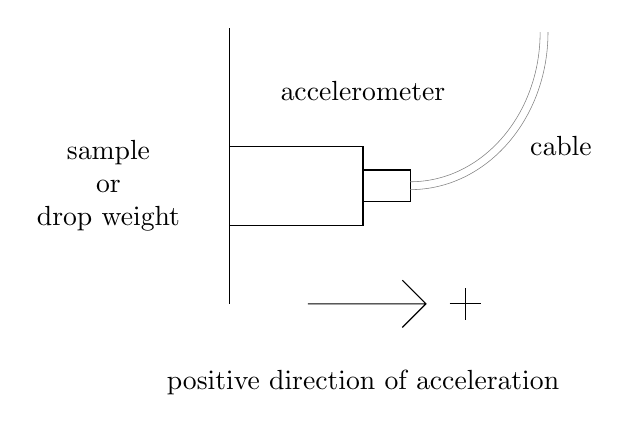
\begin{tikzpicture}

%wall
\draw (0,0.5) -- (0,1.5) 
(0,2.5) -- (0,4)

%accelerometer
(0,1.5) rectangle (1.7,2.5)
(1.7,1.8) rectangle (2.3,2.2);

%cable
\draw [help lines]
(2.3,1.95) arc [x radius = 1.75cm, y radius = 2cm, start angle= -90, end angle= 0]
(2.3,2.05) arc [x radius = 1.65cm, y radius = 1.9cm, start angle= -90, end angle= 0];

%text
\node at (1.7,3.2) {accelerometer};
\node at (3.7,2.5) [right] {cable};
\node at (-0.5,2) [left, align = center] {sample \\ or \\ drop weight};

%direction of positive acceleration
    %arrow
\draw
(1,0.5) -- (2.5,0.5)
(2.2,0.8) -- (2.5,0.5) -- (2.2,0.2);
    %plus
\draw (3,0.7) -- (3,0.3)
(2.8,0.5) -- (3.2,0.5);
    %text
\node at (1.7,-0.5) {positive direction of acceleration};

\end{tikzpicture}
    \caption{Local orientation of positive acceleration of accelerometer}
    \label{fig:posaccel}
\end{figure}

 \begin{figure}
     \centering
     \begin{tikzpicture}
%campaign 1 sensor array over view

% telfer
\draw
(0,0) -- (3,0) arc (90:0:1) -- ++ (0,-2) coordinate (centre);
%closed hook
(centre) -- ++ (255:0.5) arc (-195:-90:0.14)
(centre) -- ++ (285:0.5) arc (15:-90:0.14);
%open hook
\draw
(centre) -- ++ (240:0.5) arc (-210:-105:0.14)
(centre) -- ++ (300:0.5) arc (30:-65:0.14)
(centre) ++ (0.5,-0.3) node [right] {hook};
\draw[fill=red]
(1,-.25) circle [radius=0.25];
\draw (1,-1) node {rotary encoder}
(2,0.5) node {crane};


% drop weight
\draw
(3.5,-6) rectangle ++ (1,-3)
(4,-5) node {drop weight};
\draw[fill=red]
%(4.3,-5.95) circle [radius = 0.05];
(4.2,-6) -- ++ (0,.2) arc (180:0:0.1) -- ++ (0,-.2);
\draw [{Latex[length=3mm, width=1mm]}-{Latex[length=3mm, width=1mm]}] (4.9,-5.45) -- ++ (0,-1);
\draw (5.2,-5.95) node [right] {accelerometer};
\draw (4,-10) node[single arrow,draw,rotate=-90,minimum height=25pt] {};


%sample
\draw (1,-12) rectangle ++ (6,1)
(4,-11.5) node {sample};

%additional accelerometers
\begin{comment}
\draw (7,-11.75) rectangle ++ (.1,.5)
(5,-12) rectangle ++ (.5,-.1);
\draw[fill=red]
(7.15,-11.5) circle [radius = 0.05]
(5.25,-12.15) circle [radius = 0.05];
\draw [{Latex[length=3mm, width=1mm]}-{Latex[length=3mm, width=1mm]}] (7.4,-11.5) -- ++ (1,0);
\draw [{Latex[length=3mm, width=1mm]}-{Latex[length=3mm, width=1mm]}] (5.25,-12.4) -- ++ (0,-1);
\draw (7.15,-12.5) node {accelerometer};
\end{comment}

%loadcells
\draw[fill=red]
(1,-12) rectangle ++ (.5,-.5);
%(6.5,-12) rectangle ++ (.5,-.5);
\draw 
%(7,-13) node {loadcell}
(1.25,-13) node {loadcell};

%laser
\draw[fill=red]
(0,-14.75) rectangle ++ (1,-.5);
\draw [red,-{Latex[length=3mm, width=1mm]}]
(1,-15) -- (4,-15) -- (4,-12);
\draw (0.5,-14.25) node {laser};
%mirror
\draw
(3.75,-15.25) -- ++ (.5,.5)
(5,-15) node {mirror};

%high speed camera
\draw [fill = red] (-2,-12) rectangle ++ (.5,-.5)
(-1.5,-12.1) -- ++ (0.2,0.1) -- ++ (0,-0.3) -- ++ (-0.2,0.1);
\draw (-2,-13) node {high speed camera};

\end{tikzpicture}
     \caption{Side view of the initial sensor array}
     \label{fig:sencam1}
 \end{figure}
 \begin{figure}
     \centering
     \input{tikz/tikz13.tex}
     \caption{Side view of the updated sensor array}
     \label{fig:senside}
\end{figure}

Some changes on the test rig were implemented for these tests. To fix the problems with the laser sensor, reflective tape was applied to the samples. Additional accelerometers were fixed directly on the sample. An overview of the new sensor array is given in \autoref{fig:senside}. Things which were already present in the initial sensor array are coloured blue and the changes are highlighted in red. 

The additional accelerometers were screwed into steel plates that were glued on the sample. One on the underside, about 10 cm from the center and in line with a load cell and one on the side of the sample and close to the point of maximum deflection. For the first 2 samples Kistler accelerometers were used. The postive direction for each accelerometer was chosen locally according to placement. A global system was considered. But the accelerometers are uniaxial and their orientation changes unpredictably during the experiment. Pretending that they measure in the same plane seemed too idealized. The positive direction of acceleration is pointing away from the sample. See  \autoref{fig:posaccel}.

\section{2019-08 and 2019-09: TSL and Various Mesh Types}

A few more test were run in an internal investigation, see ADD CITATION.
The results of these tests are included in this analysis.

After conducting the experiments the results had to be processed and interpreted.

